\section{Questions and Problems}

\textbf{1. What are \( E_{\text{corr}} \), potential resistance, \( j_{\text{corr}} \), and CPR of both metals in the different working solutions?}

\begin{table}[h!]
\centering
\caption{Electrochemical data and CPR calculation for brass}
\label{tab:brass_parameters}
\begin{tabular}{|c|c|}
\hline
Parameter & Value \\
\hline
\( E_{\text{corr}} \) & \( -0.258 \) V \\
Potential Resistance & \( 1.36 \times 10^4 \) \( \Omega\cdot\text{cm}^2 \) \\
\( j_{\text{corr}} \) & \( 5.40 \times 10^{-6} \) A/cm\(^2\) \\
CPR & \( 4.17 \times 10^{-5} \) mm/year \\
\hline
\end{tabular}
\end{table}

\begin{table}[h!]
\centering
\caption{Electrochemical data and CPR calculation for steel}
\label{tab:steel_parameters}
\begin{tabular}{|c|c|}
\hline
Parameter & Value \\
\hline
\( E_{\text{corr}} \) & \( -0.388 \) V \\
Potential Resistance & \( 2.67 \times 10^2 \) \( \Omega\cdot\text{cm}^2 \) \\
\( j_{\text{corr}} \) & \( 8.87 \times 10^{-5} \) A/cm\(^2\) \\
CPR & \( 8.23 \times 10^{-4} \) mm/year \\
\hline
\end{tabular}
\end{table}

\vspace{0.5cm}

\textbf{2. Identify the different regions in the potentiodynamic polarization plots.}


The polarization curves can be divided into cathodic, anodic, and corrosion regions. 
The intersection of the anodic and cathodic branches defines the corrosion potential 
(\(E_{\text{corr}}\)) and the corrosion current density (\(j_{\text{corr}}\)), which are 
used to estimate the corrosion rate. Figures~\ref{fig:tafel_brass} and~\ref{fig:tafel_steel} 
show these regions for brass and steel.

\begin{figure}[ht!]
    \centering
    \begin{subfigure}{0.45\textwidth}
        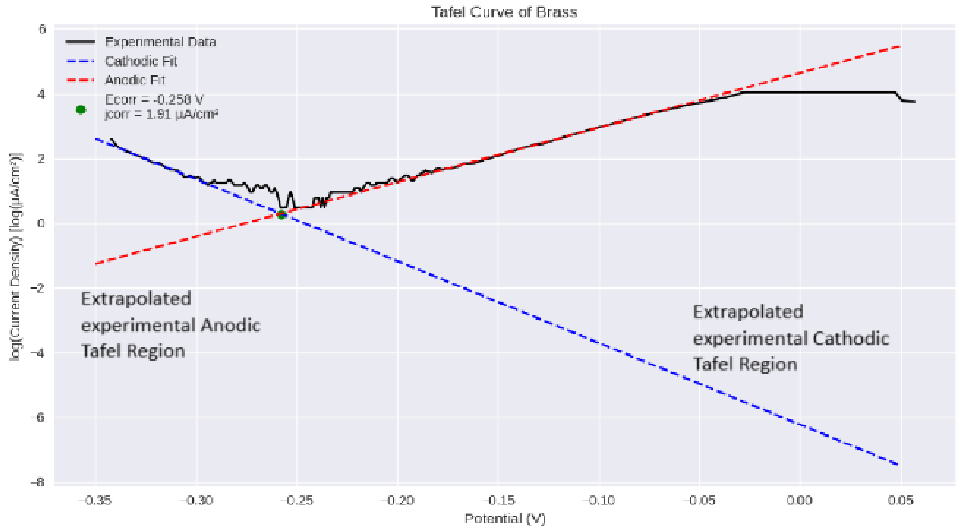
\includegraphics[width=\linewidth]{Figures/Tafel Brass.png}
        \caption{Brass Tafel plot}
        \label{fig:tafel_brass}
    \end{subfigure}
    \hfill
    \begin{subfigure}{0.45\textwidth}
        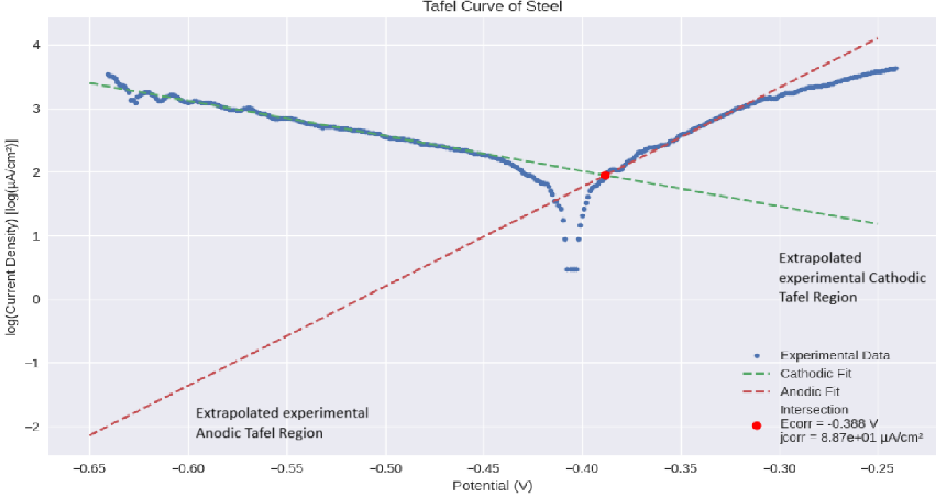
\includegraphics[width=\linewidth]{Figures/Tafel Steel.png}
        \caption{Steel Tafel plot}
        \label{fig:tafel_steel}
    \end{subfigure}
    \caption{Potentiodynamic polarization plots showing anodic, cathodic, and corrosion regions.}
\end{figure}

\vspace{0.5cm}

\textbf{3. Comparison with classmate's results}


\vspace{0.2cm}
\begin{table}[h!]
\centering
\caption{Comparison of electrochemical corrosion results between groups}
\label{tab:cpr_groups}
\begin{tabular}{|c|c|c|c|}
\hline
Group & \( E_{\text{corr}} \) [V] & \( j_{\text{corr}} \) [A/cm\(^2\)] & CPR [mm/year] \\
\hline
\textbf{JJD}  & \(-0.258\) & \( 5.40 \times 10^{-6} \) & \( 4.17 \times 10^{-5} \) \\
\hline
\textbf{GMS}  & \(-0.258\) & \( 1.6217 \times 10^{-6} \) & \( 0.11099 \) \\
\hline
\textbf{RNJM} & \(-0.186\) & \( 9.2204 \times 10^{-6} \) & \( 0.63106 \) \\
\hline
\end{tabular}
\end{table}

Comparison of the electrochemical corrosion results between the three groups reveals significant variations in corrosion kinetics (rate). The JJD and GMS groups shared the same Corrosion Potential ($E_{corr}$) of $-0.258 \text{ V}$, indicating an identical thermodynamic tendency to corrode, which is more negative than that of the RNJM group ($-0.186 \text{ V}$). However, the Corrosion Penetration Rate (CPR), which is the practical rate metric, was drastically different. The RNJM group exhibited the highest corrosion rate with an $i_{corr}$ of $9.2204 \mu\text{A}/\text{cm}^2$ and a CPR of $0.63106 \text{ mm/year}$. At the other extreme, the JJD group showed the best corrosion resistance with the lowest CPR of only $4.17 \times 10^{-5} \text{ mm/year}$, despite its more negative potential.
The large dispersion that exists between the recorded data could be due to the limitations of the equipment used, in addition to the preparation of the sample among other systematic or human errors.



\vspace{0.5cm}

\textbf{4. Comparison with literature values}

Experimental studies on steel corrosion in 0.5 M HCl report \( j_{\text{corr}} \) values typically ranging from \( 10^{-5} \) to \( 10^{-3} \) A/cm\(^2\), depending on steel type, surface condition, temperature, and inhibitor presence. According to Laamari et al.~\cite{laamari_2011_corrosion}, this range is consistent with the measured value for steel (\( 8.87 \times 10^{-5} \) A/cm\(^2\)), confirming its plausibility~\cite{loveday_electrochemical}.

For brass, the measured \( j_{\text{corr}} = 5.4 \times 10^{-6} \) A/cm\(^2\) indicates low corrosivity. Literature reports, such as those by Radovanović et al.~\cite{radovanovi_2019_electrochemical}, show that brass corrosion in HCl is highly sensitive to time, composition, and experimental setup. Differences between literature and experimental results may stem from alloy composition, surface roughness, or environmental factors.

\vspace{0.5cm}

\textbf{5. Would you expect iron to corrode in high-purity water? Why or why not?}

In high-purity water, iron exhibits a very low corrosion rate due to minimal ionic conductivity and the formation of passive oxide/hydroxide films that inhibit anodic dissolution. Additionally, the absence of dissolved oxygen suppresses cathodic reactions, resulting in negligible corrosion. However, trace amounts of oxygen or salts can disrupt passivation and significantly accelerate corrosion.

\vspace{0.5cm}

\textbf{6. Electrochemical behavior of magnesium in different solutions}

\textbf{A) Write the possible oxidation and reduction half-reactions for magnesium in the following media:}

\vspace{0.3cm}
\textbf{(i) HCl solution}



\[
\text{Overall: } \mathrm{Mg}_{(s)} + 2\mathrm{HCl}_{(aq)} \rightarrow \mathrm{Mg}^{2+}_{(aq)} + 2\mathrm{Cl}^{-}_{(aq)} + \mathrm{H}_2\mathrm{(g)}
\]




\[
\text{Oxidation: } \mathrm{Mg}_{(s)} \rightarrow \mathrm{Mg}^{2+}_{(aq)} + 2e^-
\]




\[
\text{Reduction: } 2\mathrm{H}^{+}_{(aq)} + 2e^- \rightarrow \mathrm{H}_2\mathrm{(g)}
\]



\vspace{0.3cm}
\textbf{(ii) HCl solution with dissolved oxygen}



\[
\text{Overall: } 2\mathrm{Mg}_{(s)} + \mathrm{O}_2\mathrm{(g)} + 2\mathrm{H}_2\mathrm{O}_{(l)} \rightarrow 2\mathrm{Mg}^{2+}_{(aq)} + 4\mathrm{OH}^{-}_{(aq)}
\]




\[
\text{Oxidation: } 2\mathrm{Mg}_{(s)} \rightarrow 2\mathrm{Mg}^{2+}_{(aq)} + 4e^-
\]




\[
\text{Reduction: } \mathrm{O}_2\mathrm{(g)} + 2\mathrm{H}_2\mathrm{O}_{(l)} + 4e^- \rightarrow 4\mathrm{OH}^{-}_{(aq)}
\]



\vspace{0.3cm}
\textbf{(iii) HCl solution with dissolved oxygen and Fe\(^{2+}\) ions}



\[
\text{Overall: } \mathrm{Mg}_{(s)} + \frac{1}{2}\mathrm{O}_2\mathrm{(g)} + 2\mathrm{H}_2\mathrm{O}_{(l)} + \mathrm{Fe}^{2+}_{(aq)} \rightarrow \mathrm{Mg}^{2+}_{(aq)} + 4\mathrm{OH}^{-}_{(aq)} + \mathrm{Fe}_{(s)}
\]




\[
\text{Oxidation: } \mathrm{Mg}_{(s)} \rightarrow \mathrm{Mg}^{2+}_{(aq)} + 2e^-
\]




\[
\text{Reduction 1: } \mathrm{Fe}^{2+}_{(aq)} + 2e^- \rightarrow \mathrm{Fe}_{(s)}
\]




\[
\text{Reduction 2: } \frac{1}{2}\mathrm{O}_2\mathrm{(g)} + 2\mathrm{H}_2\mathrm{O}_{(l)} + 2e^- \rightarrow 4\mathrm{OH}^{-}_{(aq)}
\]



\vspace{0.5cm}

\textbf{B) In which solution would magnesium oxidize most rapidly? Why?}

Magnesium is expected to oxidize most rapidly in the HCl solution containing both dissolved oxygen and Fe\(^{2+}\) ions. These species act as strong oxidizing agents, enhancing cathodic reactions and accelerating the overall corrosion rate. The presence of multiple electron acceptors increases the electrochemical driving force for magnesium dissolution.

